\chapter{}
\section{模型拟合}

假设数据$(x,y)$由函数$y=G(x;0,1) + G(x; 1.5, 1) + z$ 产生,其中$G(x; a,b) = \frac{1}{b\sqrt[]{2\pi}} \exp (-\frac{(x-a)^2}{2b^2})$
表示均值为$a$方差为$b$的高斯函数。$z$为均值0,方差$h$的噪声。对$x \in [0,4]$均匀采样$N$个点,生成$N$个数据对$(x,y)$,随机取其中80\%作为训练集, 10\%作为验证集,10\%为测试集。

答:首先生成数据,代码如下

\begin{python}
import random

import numpy
import numpy as np
from scipy.optimize import curve_fit
import pylab as plt

N = 100
h = 0.001


def g(x1, a, b):
    return 1 / (b * np.sqrt(2 * np.pi)) * np.exp(-(x1 - a) ** 2 / (2 * b ** 2))


def y(x1):
    return g(x1, 0, 1) + g(x1, 1.5, 1)

X = numpy.linspace(0, 4, N).round(4)
Y = y(X) # 无噪声函数值
Yr = Y + numpy.random.normal(0, np.sqrt(h), N) #噪声

index = [a for a in range(0, N)] 
random.shuffle(index) # 随机打乱
train = [[], [], []] #训练集
verify = [[], [], []] # 验证集
test = [[], [], []] # 测试集
for i in range(0, int(N * 0.8)): # 80%训练
    train[0].append(X[index[i]])
    train[1].append(Yr[index[i]])
    train[2].append(Y[index[i]])
for i in range(int(N * 0.8), int(N * 0.9)): # 10%验证
    verify[0].append(X[index[i]])
    verify[1].append(Yr[index[i]])
    verify[2].append(Y[index[i]])
for i in range(int(N * 0.9), int(N)):# 10%测试
    test[0].append(X[index[i]])
    test[1].append(Yr[index[i]])
    test[2].append(Y[index[i]])

\end{python}

\subsection{问题1}

 若假设模型参数未知,但模型形式(函数族)已知,则假设模型为$y = w_1G(x,; a_1, b_1) + w_2G(x;a_2,b_2)$ 其中$w_i,a_i,b_i$ 为参数,
 对训练集数据进行拟合,求解参数,然后看训练集和测试集上的RMSE,并作图。看采样点个数$N$和方差$h$对模型拟合的影响。
 看参数初始值对模型结果的影响。

 \subsubsection{求解参数}
 利用curve\_fit求解参数,某次求解得到的参数为
 \begin{python}
参数初始值为: [1, 1, 1, 1, 1, 1]
参数拟合值为: [1.9290132  0.69100712 1.29437368 0.07768478 1.90195323 0.58154741]
训练集RMSE= 0.0275
测试集RMSE= 0.0356
 \end{python}
 (参数顺序为 $w_1, a_1,b_1,w_2,a_2,b_2$)。
 图像如图\ref{fig:N100h0001}
 \begin{figure}[H]
    \begin{center}
        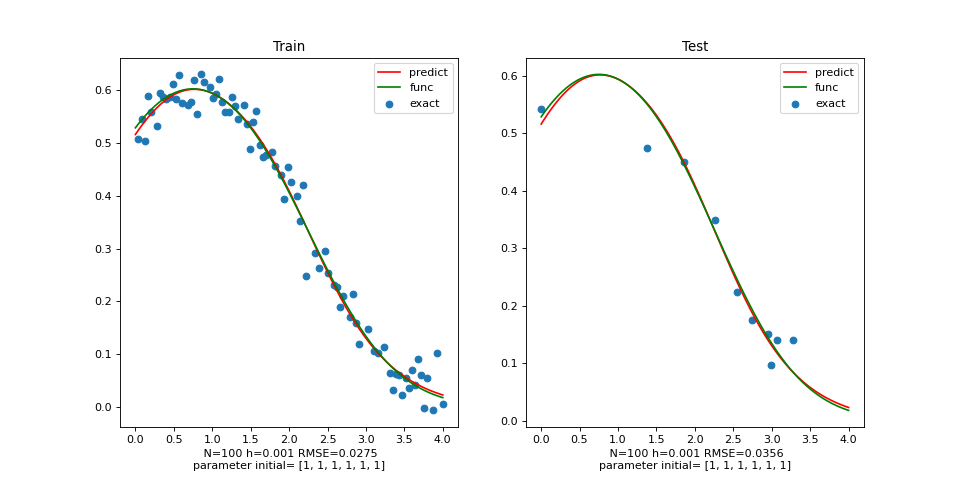
\includegraphics[width=0.9\textwidth]{img/1-N100h0001.png}
    \end{center}
   \caption[]{N100h0001}
    \label{fig:N100h0001}
\end{figure} 

 \subsubsection{采样点个数$N$和方差$h$影响}

不同$N$对于拟合带来的影响如图\ref{fig:diff-N}。可以看出,虽然不同$N$值对于训练集上的RMSE值影响不大,但对于测试集,更大的采样数$N$带量更小的误差RMSE。
\begin{figure}[H]
    \begin{center}
        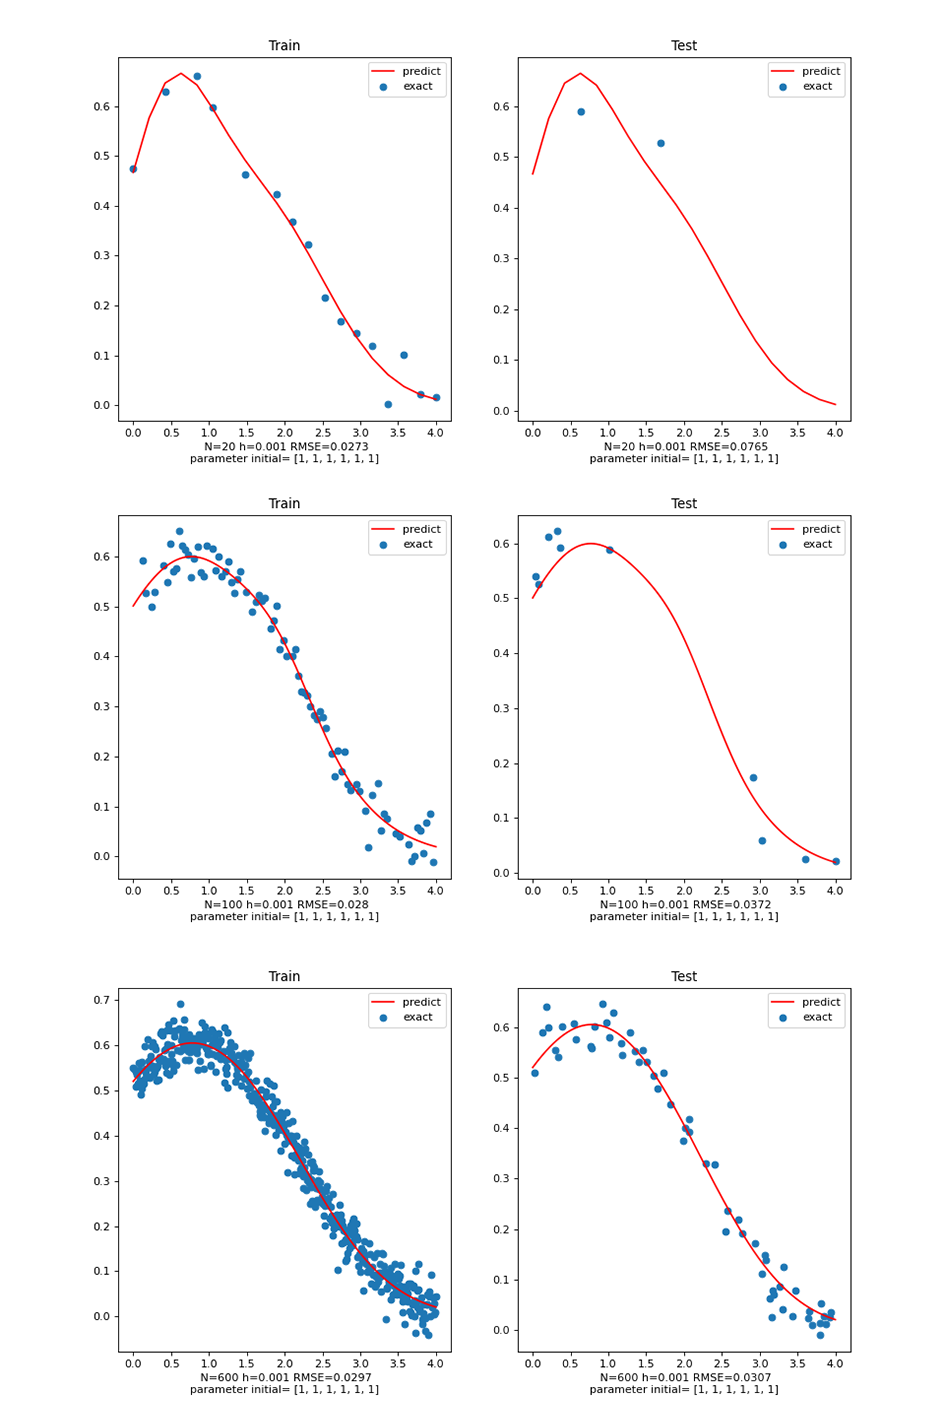
\includegraphics[width=0.9\textwidth]{img/1-diff-N.png}
    \end{center}
   \caption[]{diff-N}
    \label{fig:diff-N}
\end{figure} 

不同$h$对于拟合带来的影响如图\ref{fig:diff-h}。可以看出不论是训练集和测试机,噪声方差$h$越大,误差值RMSE值越大。

\begin{figure}[H]
    \begin{center}
        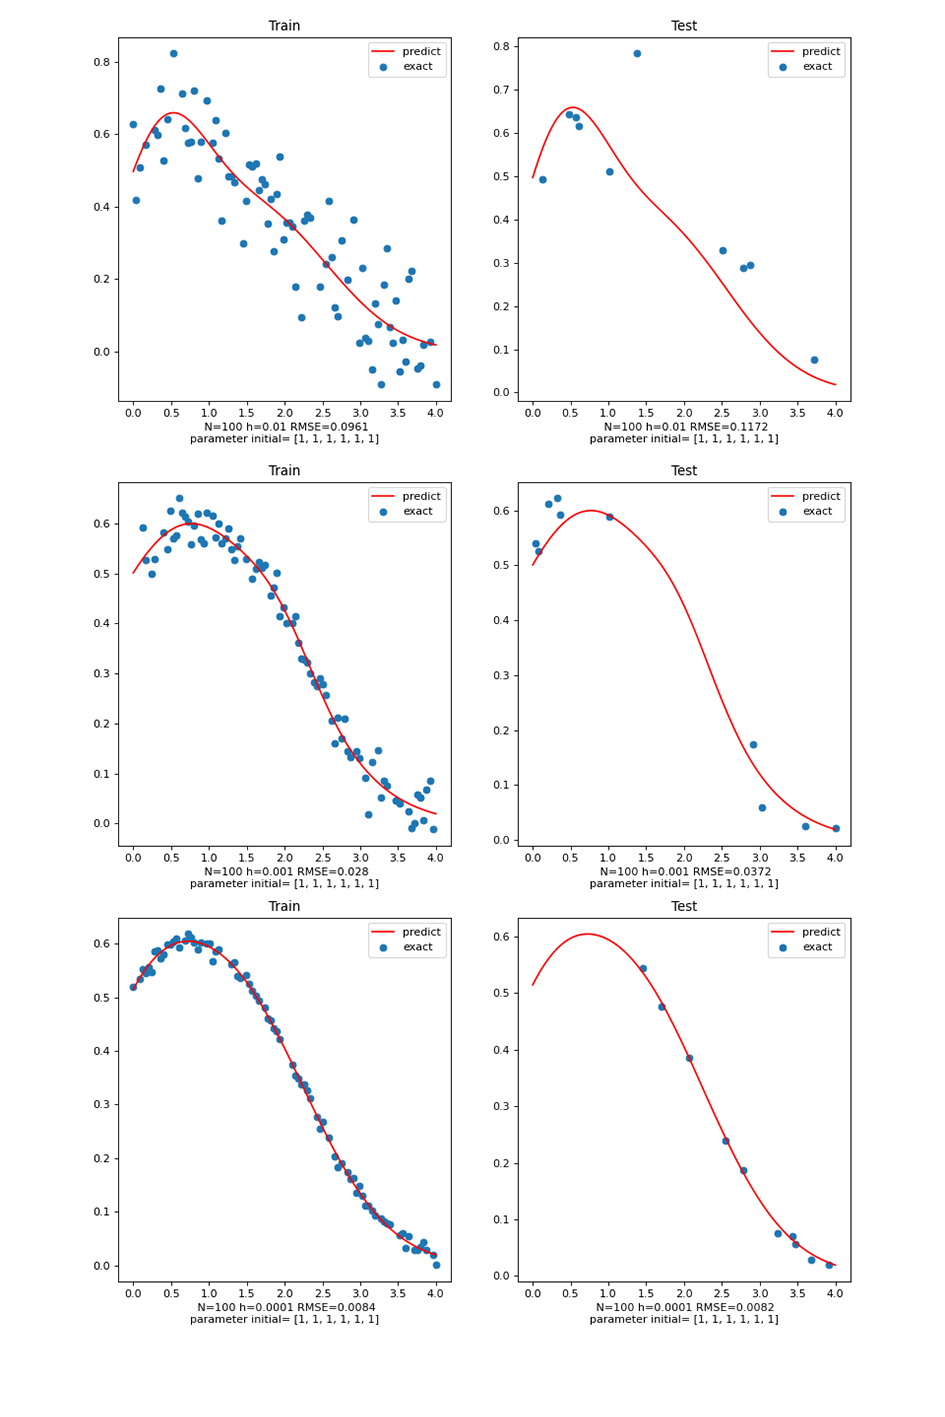
\includegraphics[width=0.9\textwidth]{img/1-diff-h.png}
    \end{center}
   \caption[]{diff-h}
    \label{fig:diff-h}
\end{figure} 

\subsubsection{参数初值影响}
    设定不同参数初值,得到结果如下
    \begin{python}
        参数初始值为: [ 0.37    1.5941  1.2558 -0.498  -0.7823  0.3197]
参数拟合值为: [ 2.40930074  0.92354962  1.58371215  0.24756718  2.90799636 -0.74886082]
训练集RMSE= 0.0288
测试集RMSE= 0.0352
参数初始值为: [1, 1, 1, 1, 1, 1]
参数拟合值为: [0.03856293 1.69769184 0.24461748 1.96918745 0.756917   1.30868267]
训练集RMSE= 0.0279
测试集RMSE= 0.0328
    \end{python}
    (参数顺序为 $w_1, a_1,b_1,w_2,a_2,b_2$)。
    画图,得到\ref{fig:diff-parameter}

    \begin{figure}[H]
        \begin{center}
            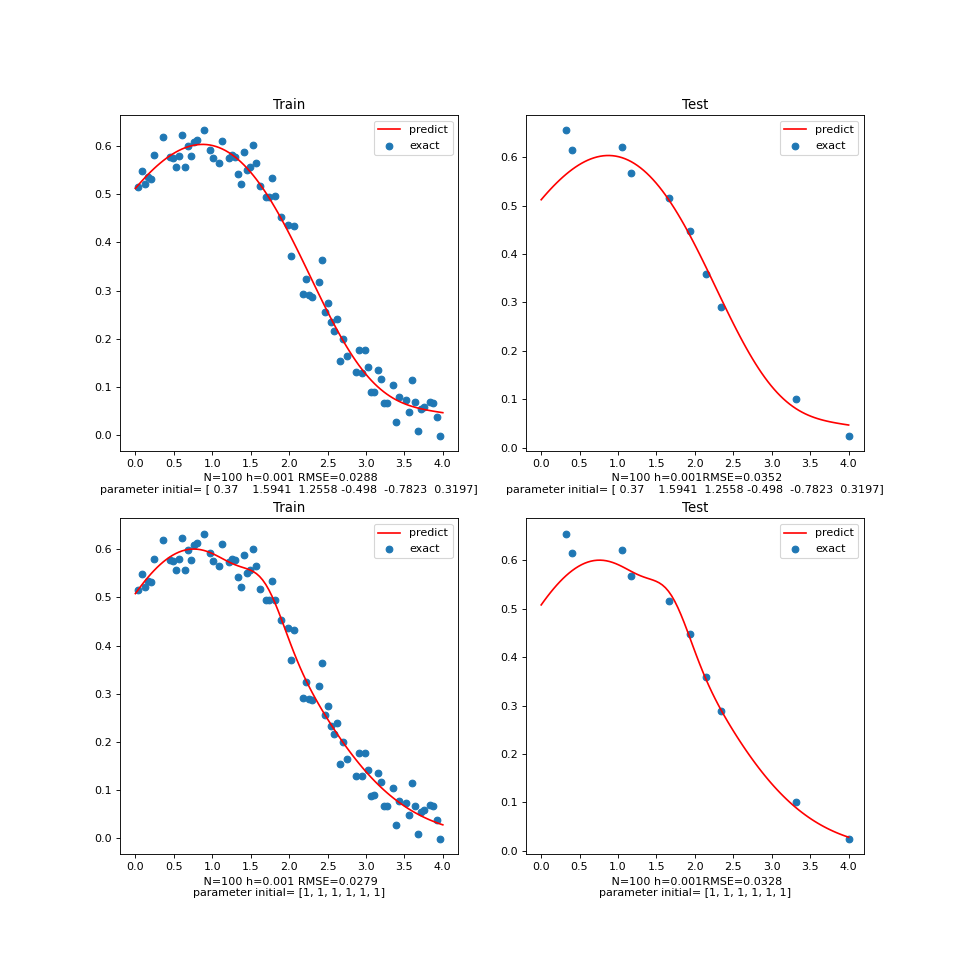
\includegraphics[width=0.9\textwidth]{img/1-diff-para.png}
        \end{center}
       \caption[]{diff-parameter}
        \label{fig:diff-parameter}
    \end{figure}

    可见不同参数初值对于模型的RMSE有影响,原因为不同的参数初值可能带来不同的优化的局部最优。

 \subsection{问题2}
 若模型形式未知,假设模型为$y = \Sigma^k_{i=0} a_ix^i$ 其中$\{a_i\}^K_{i=0}$ 为参数,
 对训练集数据进行拟合,求解参数,
 然后看训练集和测试集上的RMSE,并作图。
 看采样点个数$N$和方差$h$、模型超参数$K$对模型拟合的影响。
 看参数初始值对模型结果的影响。

 \subsubsection{求解参数}
 利用curve\_fit求解参数,某次求解得到的参数为
 \begin{python}
参数初始值为: [-3.16108138 -0.65466178  1.70021195 -0.86351663]
参数拟合值为: [ 0.49782277  0.34518524 -0.27614233  0.04031836]
训练集RMSE= 0.0332
测试集RMSE= 0.0219
 \end{python}
(参数顺序为 $a_0, a_1,a_2,a_3$)。
 图像如图\ref{fig:2-K3}
 \begin{figure}[H]
    \begin{center}
        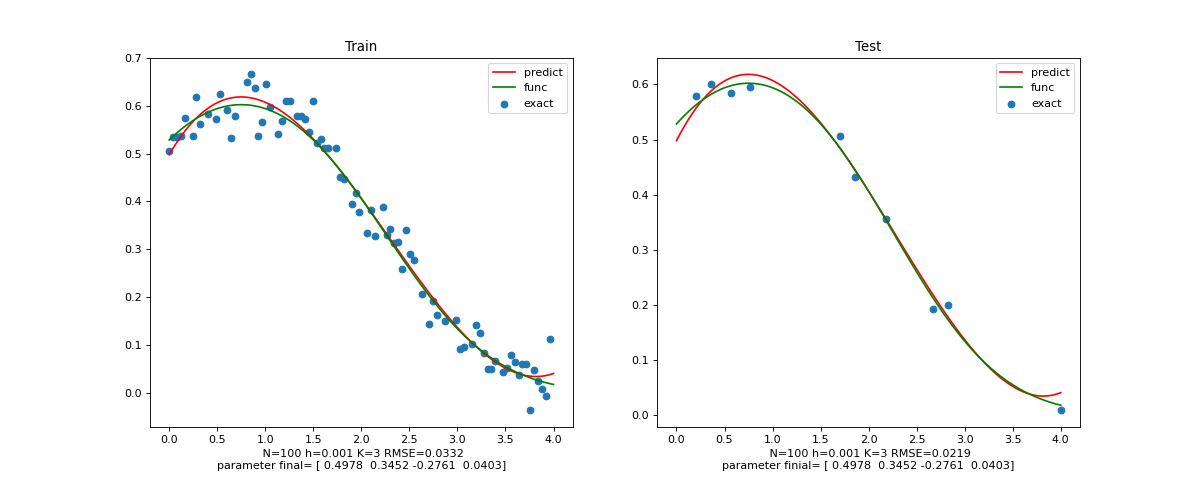
\includegraphics[width=0.9\textwidth]{img/2-K3N100.png}
    \end{center}
   \caption[]{2-K3}
    \label{fig:2-K3}
\end{figure} 

\subsubsection{不同超参数$K$值}

不同$K$对于拟合带来的影响如图\ref{fig:diff-K}。可以看出$K$过大或过小均导致模型精确度变低,
$K$过小时不能准确反应变化,$K$过大则对变化过于灵敏,存在过拟合的问题。

\begin{figure}[H]
    \begin{center}
        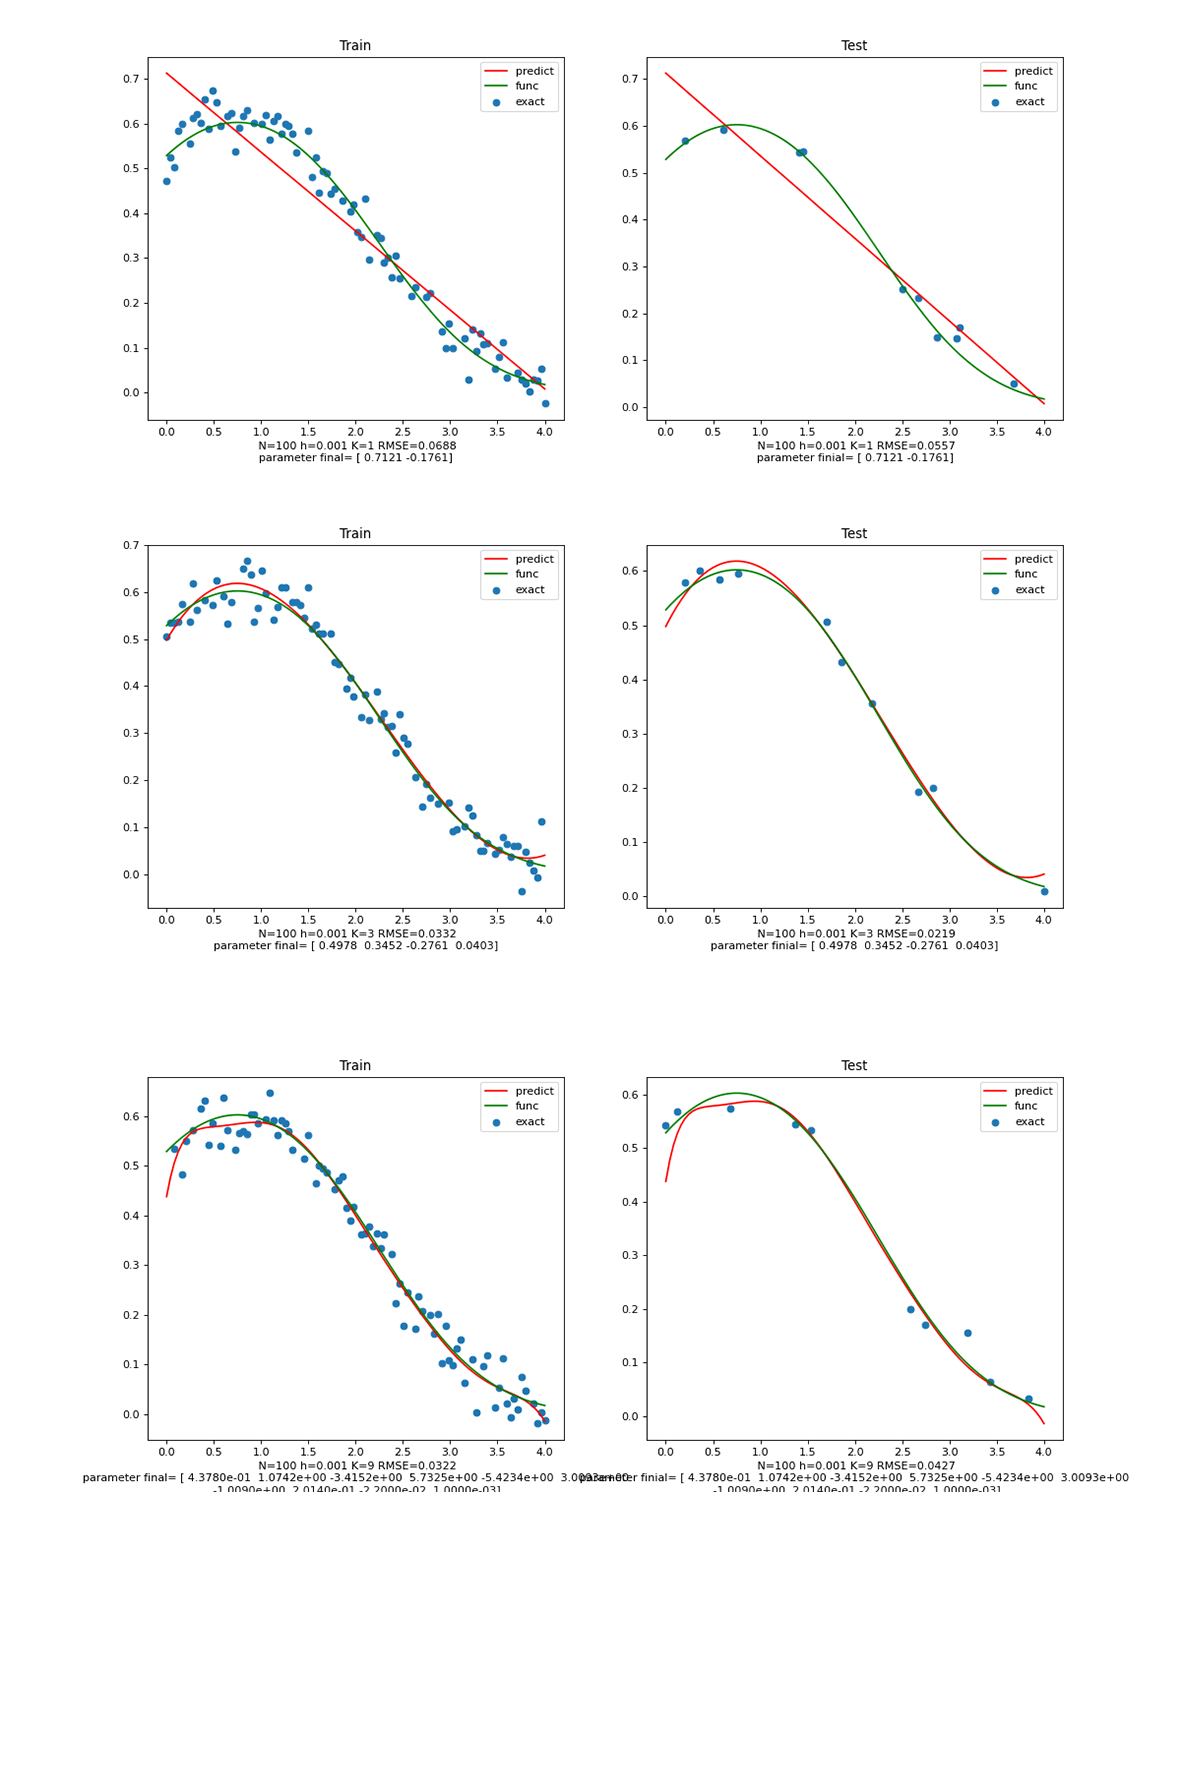
\includegraphics[width=0.9\textwidth]{img/2-diff-K.png}
    \end{center}
   \caption[]{diff-K}
    \label{fig:diff-K}
\end{figure} 

\subsubsection{不同$N$和$h$}

不同$N$和$h$下的情况与第一问大致类似,值得一提的是,在$N$较小,$K$较大时,过拟合问题更加明显,如图\ref{fig:2-K9N20}。

\begin{figure}[H]
    \begin{center}
        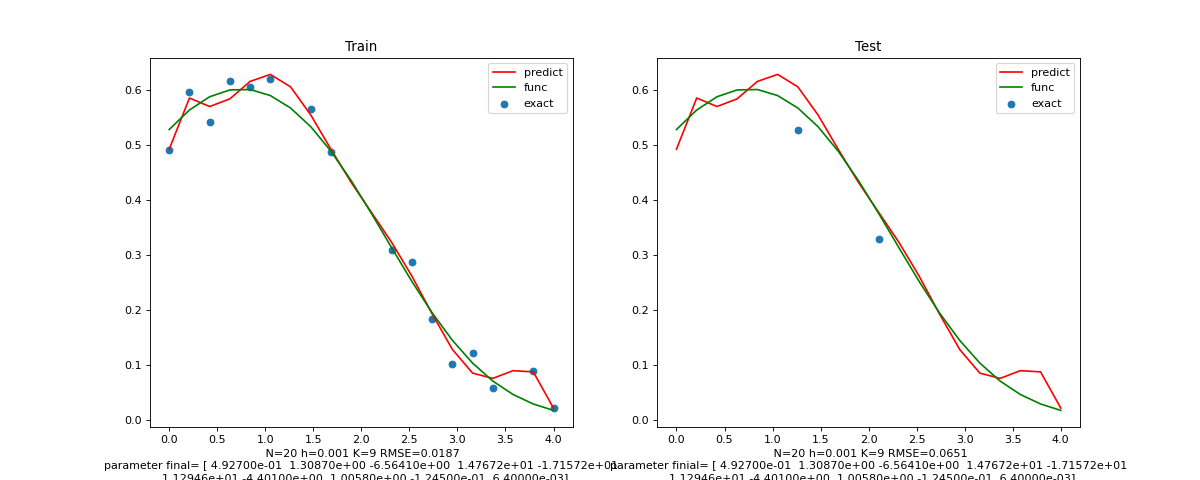
\includegraphics[width=0.9\textwidth]{img/2-K9N20.png}
    \end{center}
   \caption[]{2-K9N20}
    \label{fig:2-K9N20}
\end{figure} 

\subsubsection{不同参数初始值}

不同参数初始值下的情况与问题一大致类似。

 \subsection{问题3}
 若模型形式未知,假设模型为$y=\Sigma^K_{i=0}\Sigma^M_{j=0} w_{ij}x^jG(x;a_i,b_i)$,其中$\{w_{ij}, a_i, b_i\}$ 为参数,
 对训练集数据进行拟合,求解参数,
 然后看训练集和测试集上的RMSE,并作图。
 看采样点个数$N$和方差$h$、模型超参数$K$和$M$对模型拟合的影响。
 看参数初始值对模型结果的影响。

 \subsubsection{求解参数}
 利用curve\_fit求解参数,某次求解得到的参数为
 \begin{python}
    参数拟合值为: [-2.90721005e+00  6.51344613e-01 -3.14073751e+02 -1.46424351e+04
  1.36713804e+00 -1.44028058e+00 -1.21483365e+01  1.38207755e+00]
训练集RMSE= 0.0313
测试集RMSE= 0.0167
 \end{python}
 (参数顺序为 $w_00, w_01, w_10, w_11, a_0, b_0, a_1, b_1$)

 图像如图\ref{fig:3-K1M1N100}
 \begin{figure}[H]
    \begin{center}
        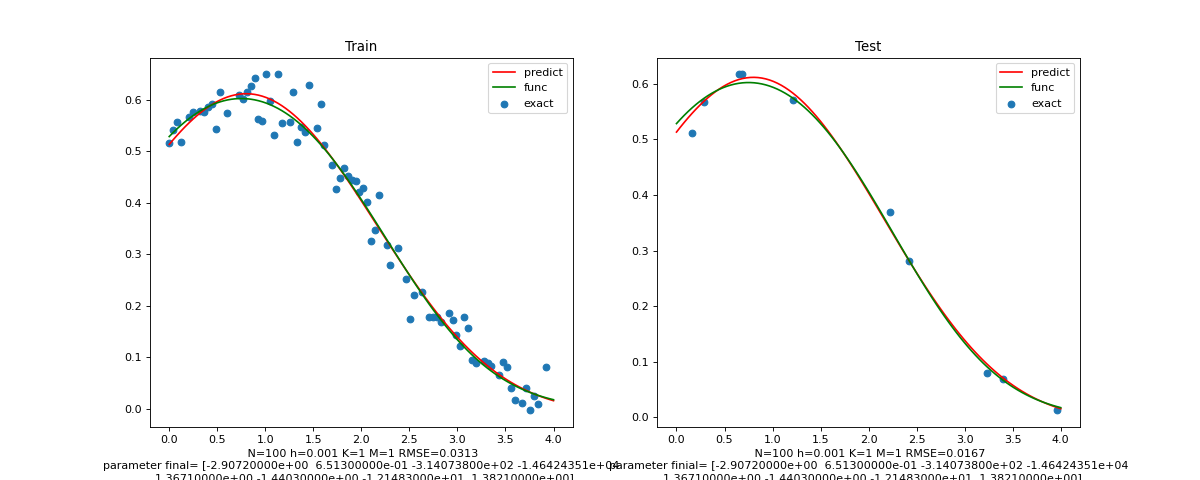
\includegraphics[width=0.9\textwidth]{img/3-K1M1N100.png}
    \end{center}
   \caption[]{3-K1M1N100}
    \label{fig:3-K1M1N100}
\end{figure} 

\subsubsection{不同$N$和$h$}

不同$N$和$h$下的情况与第一问大致类似。

\subsubsection{不同超参数$K$和$M$}

不同$K$和$M$对于拟合带来的影响如图\ref{fig:diff-KM}。当$K=1,M=1$时模型较好。

\begin{figure}[H]
    \begin{center}
        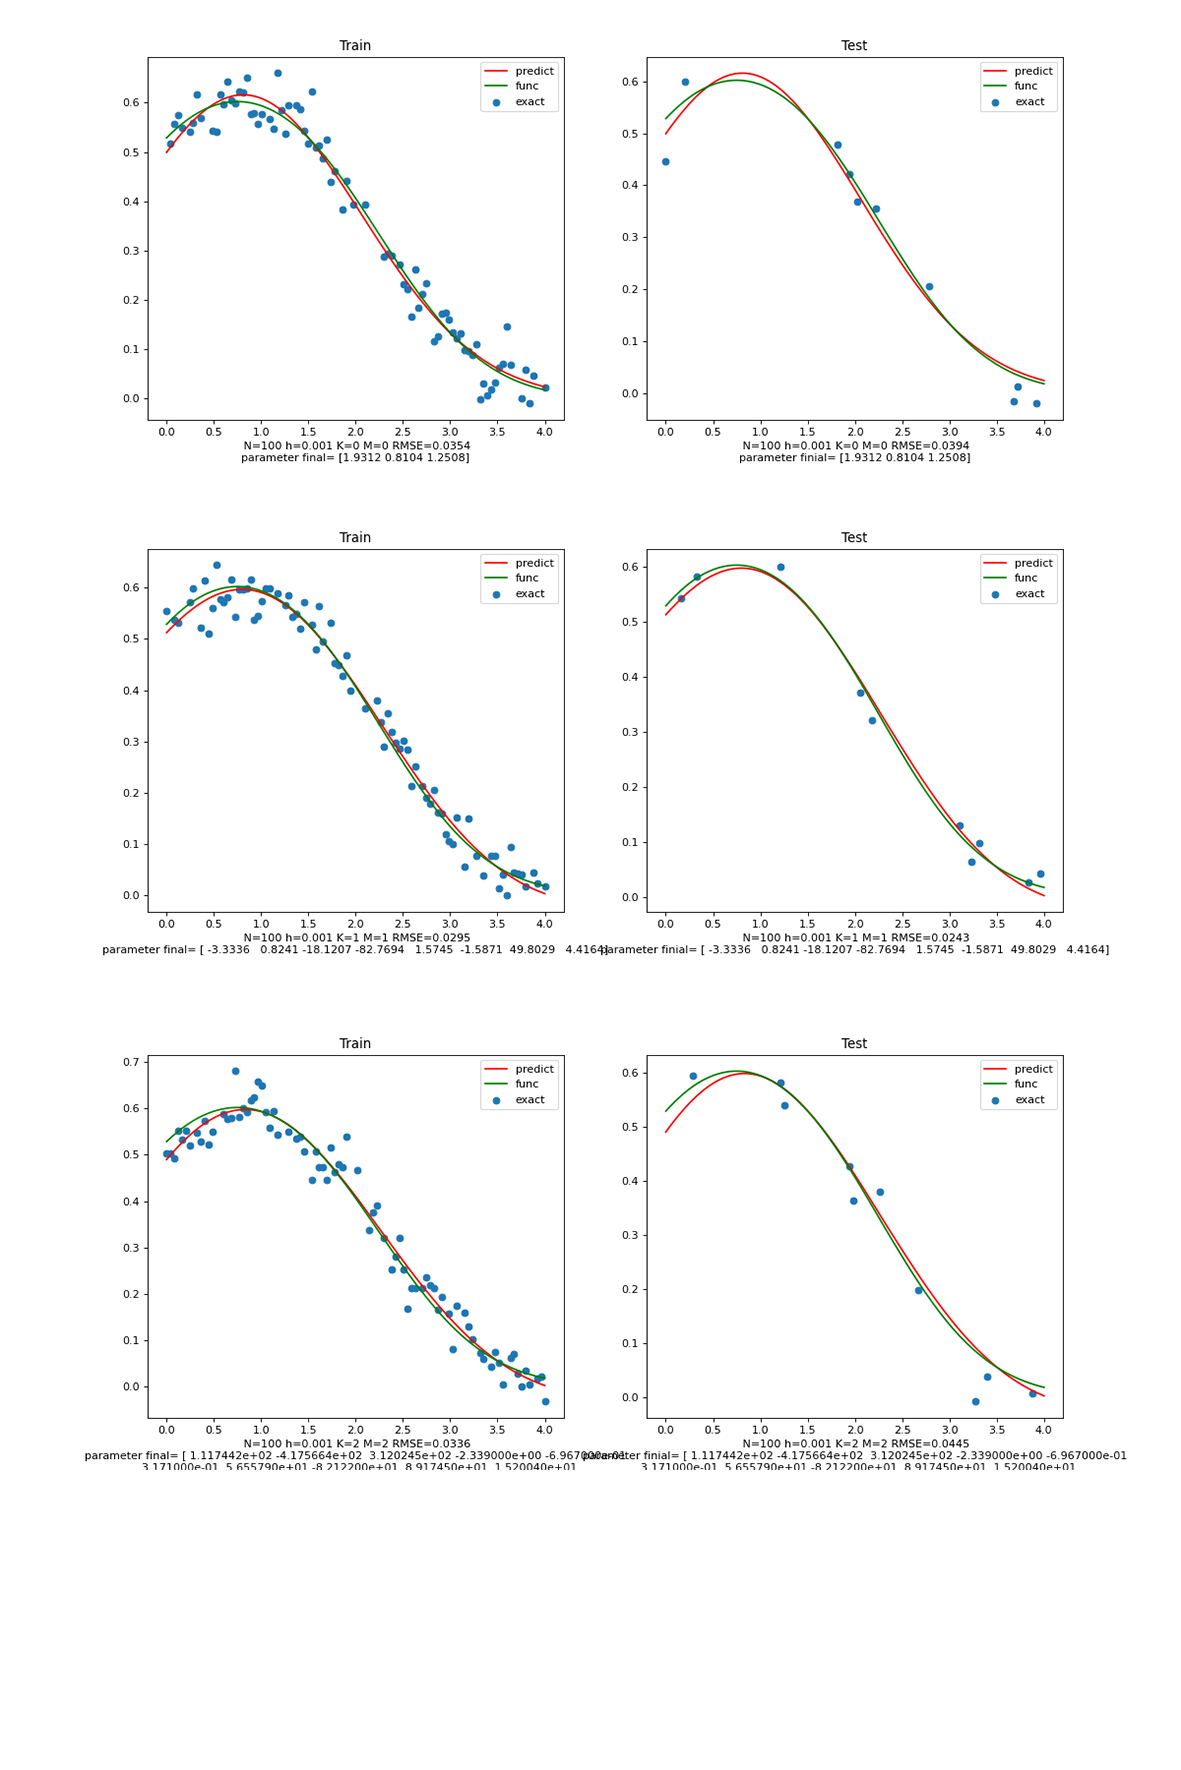
\includegraphics[width=0.9\textwidth]{img/3-diff-KM.png}
    \end{center}
   \caption[]{diff-KM}
    \label{fig:diff-KM}
\end{figure} 

\subsubsection{不同参数初始值}

不同参数初始值的情况与问题一类似。


 \subsection{问题4}

 若模型形式未知,假设模型为$y=a \cos (bx) + c$,其中$\{a,b,c\}$ 为参数,
 对训练集数据进行拟合,求解参数,
 然后看训练集和测试集上的RMSE,并作图。
 看采样点个数$N$和方差$h$、模型超参数$K$和$M$对模型拟合的影响。
 看参数初始值对模型结果的影响。
 设 $b=10000$, 拟合模型求$a$和$c$看结果如何,RMSE在训练集,验证集, 和测试集有什么变化。
 
 \subsubsection{求解参数}
 利用curve\_fit求解参数,某次求解得到的参数为
 \begin{python}
参数初始值为: [-1.51116033 -1.30828028 -0.81722307]
参数拟合值为: [ 0.37334812 -0.58239804  0.24416905]
训练集RMSE= 0.0461
测试集RMSE= 0.0373
验证集RMSE= 0.276
 \end{python}
 (参数顺序为 $a,b,c$)

 图像如图\ref{fig:4-N100}
 \begin{figure}[H]
    \begin{center}
        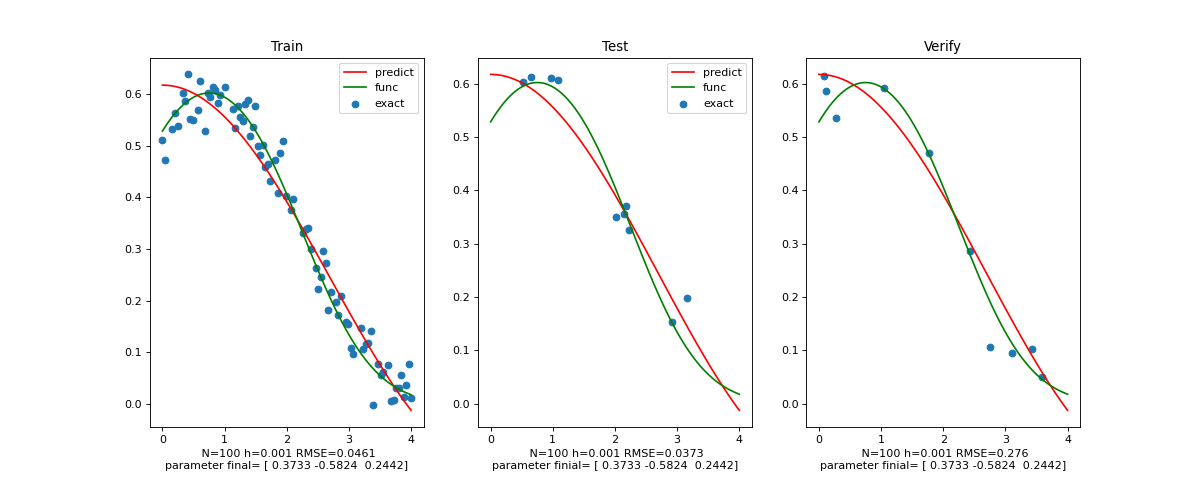
\includegraphics[width=0.9\textwidth]{img/4-N100.png}
    \end{center}
   \caption[]{4-N100}
    \label{fig:4-N100}
\end{figure} 

\subsubsection{固定b,求解a/c}

求解得
\begin{python}
参数初始值为: [1, 1]
参数拟合值为: [-0.021126   0.3583394]
训练集RMSE= 0.2134
测试集RMSE= 0.2276
验证集RMSE= 0.2279

\end{python}
(参数顺序为 $a,c$)

图像如图\ref{fig:4-b10000}。
\begin{figure}[H]
   \begin{center}
       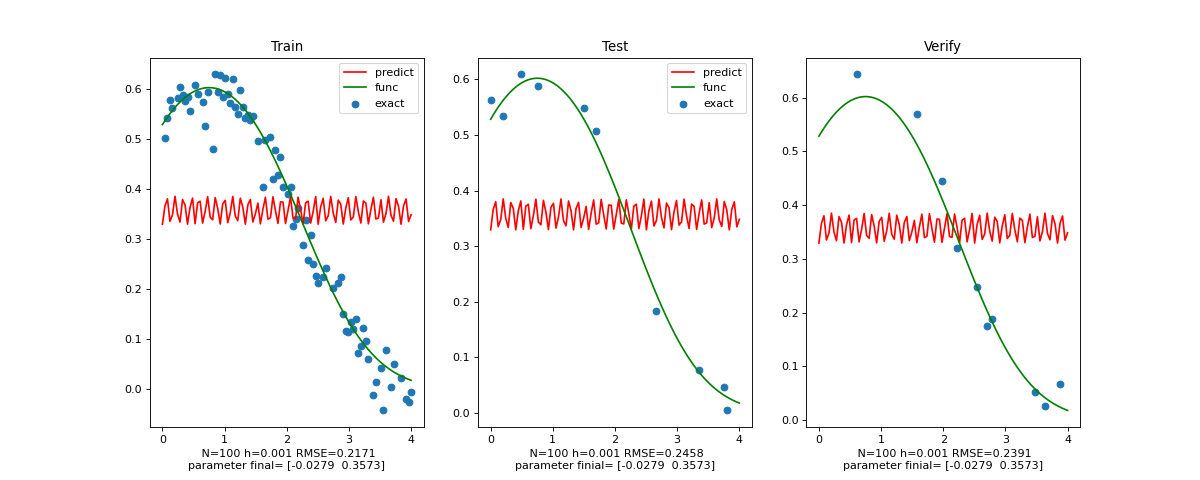
\includegraphics[width=0.9\textwidth]{img/4-b10000.png}
   \end{center}
  \caption[]{4-b10000}
   \label{fig:4-b10000}
\end{figure} 

可以发现参数$c$大致不变,但参数$a$明显变小,并且模型的准确度十分差。

\subsubsection{不同$N$和$h$}

不同$N$和$h$下的情况与第一问大致类似。

\subsubsection{不同参数初始值}

不同参数初始值的情况与问题一类似。值得一提的是,在固定$b=10000$的情况下,$a$需要选择0附近的初始值,不然优化时间会过长。


 \subsection{问题5}

 上述2)、3)、4)中不同模型,利用验证集选取一个最好(RMSE最小)的模型,看它在测试集上的误差。

 答:

 从2)、3)、4)不同类别的模型中各挑选一个表现较好的进行比较。
 从2)中选择$K=3$的模型,从3)中选择$K=1,M=1$的模型,从4)中选择不限制$b$的模型,在验证集上计算RMSE。
 得到如下结果
\begin{python}
model2 verify RMSE= 0.0055
model3 verify RMSE= 0.0041
model4 verify RMSE= 0.0313
model2 test RMSE= 0.0118
model3 test RMSE= 0.0081
model4 test RMSE= 0.0485
\end{python}

 画图,得图\ref{fig:q5}。

 \begin{figure}[H]
    \begin{center}
        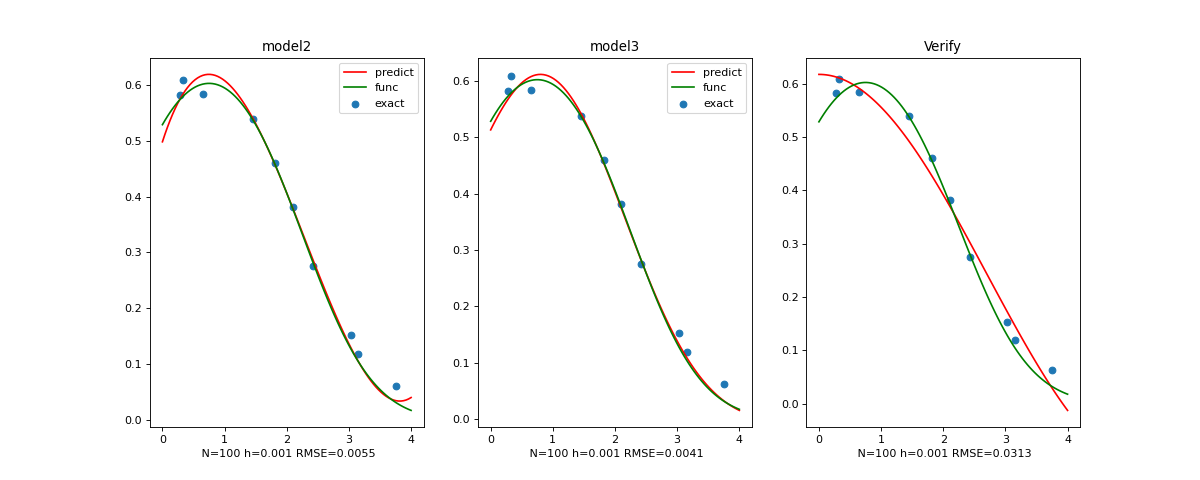
\includegraphics[width=0.9\textwidth]{img/5.png}
    \end{center}
   \caption[]{q5}
    \label{fig:q5}
 \end{figure} 

 可以看出,验证集上,模型3)中$K=1,M=1$的模型表现最好。该模型在测试集上的RMSE为0.0081。
